\documentclass[twocolumn]{article}
\usepackage{graphicx}
\usepackage{amsmath}
\usepackage{float}
\usepackage{amssymb} %Use of therefore symbol
\usepackage{hyperref}
\usepackage{caption}



\begin{document}
\title{Assignment 1: Monte Carlo Methods}
\author{Alex Matheson, Austin Nhung}
%\affiliation{Department of Physics and Astronomy, University of Calgary, Calgary AB T2N 1N4 Canada}
\date{\today}
\maketitle

\section{Introduction}
Randomness is a concept central to many processes of modern physics. Random methods however, have been developed not just to simulate random processes, but to efficiently solve or approximate intricate, deterministic processes. This assignment will expand upon the concepts demonstrated in lab 1 to provide examples of how random techniques may be used to solve physical problems. Five sub-areas of randomness were examined in this assignment: the generation of random numbers, forecasting with Markov Chains, Monte Carlo methods, annealing modifications to Monte Carlo, and traveling salesman algorithms. The examples illustrated in this assignment range from more mathematical problems to real-world applications in business.

\section{Methods}
\subsection{Random Numbers}
A classic example when considering randomness and combinations was the birthday problem. In this problem, a room of people is more likely to contain two people with the same birthday than might seem reasonable by intuition. Within a room with $35$ people, the number of pairings possible was:
\begin{equation}
N_{pairs} = \frac{30!}{28!*2!} = \frac{30*29}{2} = 435
\end{equation}
For each of these possible pairings, the probability that two people have different birthdays was $\frac{364}{365}$. This probability then needed to be taken 435 times:
\begin{equation}
\bigg( \frac{364}{365} \bigg)^{435} = 0.303
\end{equation}

Hence, there was a $30.3\% $ chance of no-one in the room having the same birthday, or a $69.7\%$ chance that at lease two people in the room had the same birthday. Code was written in fortran 90 to test this derivation. A test was run for a single room of people. An array of 30 random birthdays was created, and then each birthday compared to the others to determine if at least one pair matched. In this test, there was a pair of birthdays. After this code was run for $10,000$ loops, 6989 loops were found to have a pair of matching birthdays. Where this was close to the analytic solution above, it was assumed that analytic and computational solutions matched, and the analysis was correct.

The accept / reject method is a way to geometrically sample from a probability distribution. This method was tested on a Gaussian distribution with mean $\mu=5$ and standard deviation $\sigma=1.25$. In order to simplify the writing of code, a proposal distribution was chosen that was a uniform step between $y=0$ and $y=10$. The height of this distribution was chosen to be the maximum of the Gaussian distribution. A Gaussian distribution has a maximum at the mean value, resulting in a peak of size $(2 \pi \sigma^2)^{\frac{-1}{2}} = 0.356$. 

The code was run for $10^6$ iterations to create a distribution along $y$ matching a Gaussian distribution. Figure \ref{fig:Gauss_Dist} shows the distribution obtained by the code, and by an analytical solution. As expected, the two distributions match almost exactly. Some extremely small deviations are noted in some bins, however this would likely diminish with further samples. Alternately, these slight deviations could be improved by using a parabola or some other proposal distribution as opposed to a uniform distribution. In that case, there would be more points accepted from the $10^6$ proposed points. Another distribution was tested by summing 10 points from the above Gaussian sampler. $10^4$ sums $s$ were completed, and then the distribution of these points $s$ was plotted. Figure \ref{fig:Gauss_sum} shows the obtained distribution. Both the mean and standard deviation of the distribution were calculated and used to plot a Gaussian distribution based on those parameters. It was seen that the sum distribution was also a Gaussian. This was expected, as a Gaussian distribution is a common result of an identical experiment with an expectation value being performed multiple times.

\begin{figure}
\centering
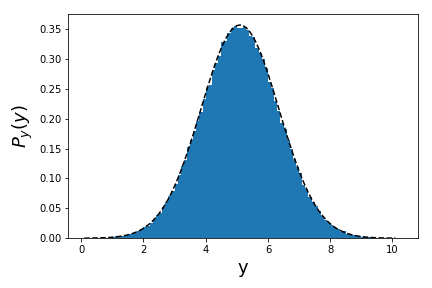
\includegraphics[width=\linewidth]{../Assn1/Gauss_Dist}
\caption{Gaussian distributions constructed from the accept/reject method (the blue histogram) and analytically (the black line). The Gaussians have mean $\mu=5$ and standard deviation $\sigma=1.25$.}
\label{fig:Gauss_Dist}
\end{figure}

\begin{figure}
\centering
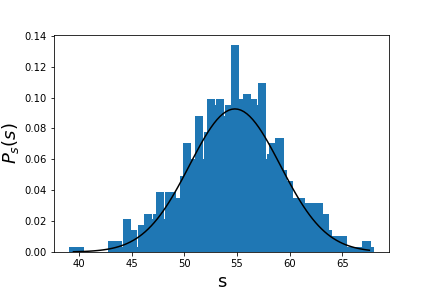
\includegraphics[width=\linewidth]{../Assn1/Gauss_sum}
\caption{Distribution of a number $s$ calculated by summing 10 numbers from a Gaussian distribution. The blue histogram shows the distribution of samples while the black line shows a Gaussian distribution constructed from parameters of the data.}
\label{fig:Gauss_sum}
\end{figure}

A cumulative distribution function (CDF) was examined as shown in table \ref{tab:CDF}. This CDF describes how long a maintenance check takes to complete. For this table, a fraction of 0.21 checks were completed in 15 minutes or less. A fraction of 0.1 takes longer than 30 minutes. Lastlt, a fraction of 0.13 checks takes between 10 and 15 minutes.

\begin{table*}[h]
\begin{center}
\begin{tabular}{|c|c|c|c|c|c|c|c|}
	\hline $t$, in minutes & 0.0 & 5.0 &10.0  &15.0  &20.0  &25.0  &30.0  \\ 
	\hline  CDF, fraction completed &0.0  &0.03  &0.08  &0.21  &0.38  &0.8  &0.9  \\ 
	\hline 
\end{tabular} 
\end{center}
\caption{Cumulative Distribution function at different times $t$.}
\label{tab:CDF}
\end{table*}

\subsection{Markov Chain}
An example provided than may be solved my Markov chain is movement between different vertices on a square with two opposite corners connected by a diagonal line. A transition matrix may be constructed describing the probability that a walker at one vertex will walk to a different vertex:
\[ P = \begin{pmatrix}
0 & 0.33 & 0.33 & 0.33 \\
0.5 & 0 & 0.5 & 0 \\
0.33 & 0.33 & 0 & 0.33 \\
0.5 & 0 & 0.5 & 0
\end{pmatrix} \]

A stable-state solution may be found analytically by separating the matrix into a series of equations and adding a fifth condition where the probability of the walker being at each vertex sums to 1. Together the equations are:
\begin{equation}
\begin{split}
3p_1 =& p_2 + p_3 + p_4 \\
2p_2 =& p_1 + p_3 \\
3p_3 =& p_1 + p_2 + p_4 \\
2p_4 =& p_1 + p_3 \\
1 =& p_1 + p_2 + p_3 + p_4
\end{split}
\end{equation}

This yields a solution of $p_1 = p_2 = p_3 = p_4 = 0.25$. Another method for finding a solution is to find the eigenvectors of the transition matrix. First, the eigenvalues of the matrix were found using the determinant method to be: $\lambda_1 = 1$, $\lambda_2 = -\frac{2}{3}$, $\lambda_3 = -\frac{1}{3}$, and $\lambda_4 = 0$. When plugging these values into the equation $PI-\lambda=0$, the following four eigenvectors were found:

\[
v_1 = \begin{pmatrix}1 \\ 1 \\ 1 \\ 1\end{pmatrix}, v_2= \begin{pmatrix}-\frac{2}{3} \\ 1 \\ -\frac{2}{3} \\ 1\end{pmatrix}, v_3= \begin{pmatrix}-1 \\ 0 \\ 1 \\ 0\end{pmatrix}, v4 = \begin{pmatrix}0 \\ -1 \\ 0 \\ 1\end{pmatrix}
\]

Since only the first eigenvector is completely positive, it is the only possible solution. When the vector is normalized, this yields the same solution as the system of equations. 

%GRAPHS GRAPHS GRAPHS GRAPHS

A more tangible example is present in the business realm. A transition matrix describes customers' liklihood of changing between different cell phone carriers:
\[
P = \begin{pmatrix}
0.80 & 0.10 & 0.10 \\
0.03 & 0.95 & 0.02 \\ 
0.20 & 0.05 & 0.75
\end{pmatrix}
\]

The three carriers have a current market share of $45\%$, $25\%$, and $30\%$. After 1 iteration of the Markov chain (1 month), the distribution of Market share is predicted to be:
\[
\begin{pmatrix}
0.80 & 0.10 & 0.10 \\
0.03 & 0.95 & 0.02 \\ 
0.20 & 0.05 & 0.75
\end{pmatrix} \begin{pmatrix} 0.45 \\ 0.25 \\ 0.30 \end{pmatrix} = \begin{pmatrix} 0.415 \\ 0.2575 \\ 0.3275 \end{pmatrix}
\]

And after two months:
\[
\begin{pmatrix}
0.80 & 0.10 & 0.10 \\
0.03 & 0.95 & 0.02 \\ 
0.20 & 0.05 & 0.75
\end{pmatrix} \begin{pmatrix} 0.415 \\ 0.2575 \\ 0.3275 \end{pmatrix} = \begin{pmatrix} 0.41625 \\ 0.25773 \\ 0.415 \end{pmatrix}
\]

Using the same analytical eigenvector model as above, the normalized eigenvector for the equilibrium market distribution was $S_1 = S_2 = S_3 = 0.33$ where $S_n$ is the market share of brand $n$. The equilibrium forecast should not be confused for the actual distribution of a product in the future. This is because the problem is probabilistic by nature: there is an $80\%$ chance that a customer will not change brands. This is not the same as saying that $80\%$ of customers in a given month will not change brands, unless the number of customers is obscenely high. The example from the previous lab better illustrated this aspect of Markov chains. Consider a matrix representing weather forecasts. In such an example, the weather was binary: either the day was sunny or rainy. The system eventually reached an equilibrium of $0.86$ sun, however the system can only have states $0$ or $1$ for whether or not the state is sunny.The business example contains two statistical characteristics rolled into one vector: the probability of a single customer using that brand, and the probability of a customer at the initial state using that brand.

\subsection{Markov Chain Monte Carlo}
 Markov chain Monte Carlo is a method of sampling a distribution using random walkers governed by a Markov chain instead of by geometric sampling. A PDF was provided to sample from using both methods. The relevant PDF was a simple Gaussian:
 \begin{equation}
 \omega(x) = exp(-0.2x^2)
 \label{lilgauss}
 \end{equation}
 
 A fortran 90 code was written to generate a distribution using the Markov chain method. The method was allowed to run for 5000 iterations in order to obtain a representative sample. A distribution provided by this method was not accurate right away, as the algorithm requires time for the random walker to reasonably be able to walk to all areas of the distribution. In order to visualize this burn-in time, the values generated by the algorithm and the mean of the distribution up to that point were recorded at each step. Figure \ref{fig:MCMCmean} shows both the values generated and the rolling mean at each iteration. By looking at the figure, the mean appeared to stabilize after a burn-in of 250 iterations. 
 
 \begin{figure}
\centering
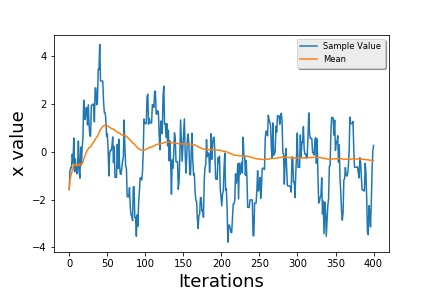
\includegraphics[width=\linewidth]{MCMCmean}
\caption{First 400 values generated by a Markov chain Monte Carlo algorithm. The mean of the proceeding values is tracked by the orange line. The mean asymptotically approaches the expected mean of $x=0$ over time. Random steps were selected using a uniform distribution from $(-\sigma, \sigma)$ where $\sigma$ was the standard distribution of the Gaussian distribution being sampled.}
\label{fig:MCMCmean}
\end{figure}

\begin{figure}
\centering
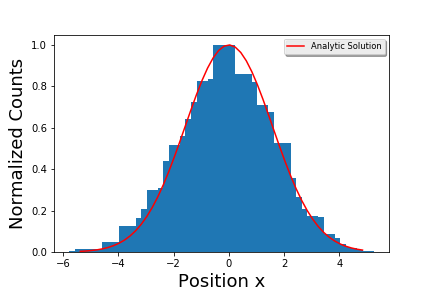
\includegraphics[width=\linewidth]{MCMChisto}
\caption{Distribution of a 5000 sample Gaussian sampling. Samples were drawn from the distribution in equation \ref{lilgauss}.}
\label{fig:MCMChisto}
\end{figure}

The same distribution was sampled using the accept/reject method to compare to the Markov chain Monte Carlo results. The accept/reject method was significantly slower, requiring $152s$ to complete as opposed to the $7.81E-02s$ required for the Markov method. To ensure a faithful comparison, the accept/reject set was required to compute until it found a distribution of 5000 points, instead of merely 5000 tests. Because any given iteration has a chance to be rejected, the accept/reject method is less efficient. In the fortran code, a uniform distribution based on the peak height was used. While choosing a proposal distribution with less rejectable space would speed up the acceptance algorithm, there would always be some rejections, making Markov methods better for large samplings.

The Metropolis-Hastings algorithm is a more sophisticated version of Markov Chain Monte Carlo that takes into account the sampling of random steps. To provide an example of this method, the following PDF was considered:
\begin{equation}
P(x) = Cx^{-5/2}e^{-\frac{2}{x}}
\label{PDF}
\end{equation}

In the case of a symmetric distribution, the acceptance probability is simply that of a standard Metropolis algorithm. Take for instance a proposal value $x^* = 39.82$ from an $x_n=0.0$. It would have an acceptance value of:
\begin{equation}
\begin{split}
A(x_n \to x^*) =& Min \Bigg( 1, \frac{C(39.82)^{-5/2}e^{\frac{-2}{39.82}}}{C(1.0)^{-5/2}e^{\frac{-2}{1.0}}} \Bigg) \\
A(x_n \to x^*) =& Min \Bigg( 1, \frac{0.000095}{0.135} \Bigg) \\
A(x_n \to x^*) =& 0.000703
\end{split}
\end{equation}
In this case, the jump is far in the tail of the Gaussian, and is extremely unlikely to be accepted. Figure \ref{fig:PDF} shows the probability distribution function.

\begin{figure}
\centering
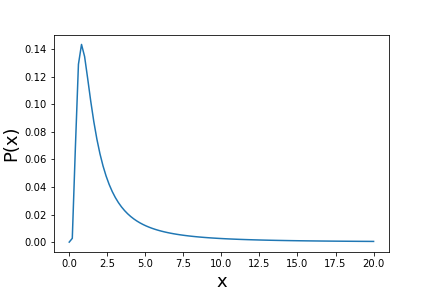
\includegraphics[width=\linewidth]{PDF}
\caption{A probability distribution function defined by equation \ref{PDF}}
\label{fig:PDF}
\end{figure}


A code was written in fortran to sample from the PDF using two different proposal distributions. First, a uniform distribution on the range $(0,100)$ was used. Next, a proposal $\chi^2$ distribution was used to sample points.

\begin{figure}
\centering
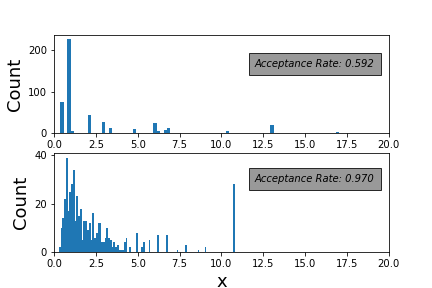
\includegraphics[width=\linewidth]{mixed_chains}
\caption{Samples from distribution \ref{PDF} using two different proposal distributions. In the upper histogram, a uniform distribution was used. In the bottom, a $\chi^2$ distribution was used. The plots were cropped from the range $(0,100)$ to $(0,30)$ to better show features near the origin. The uniform histogram has wider bins due to the high number of counts far from the origin. The $\chi^2$ histogram had an 'unlucky' spike past $x=10$ due to random draws.}
\label{fig:mixed_chains}
\end{figure}
 

\subsection{Simulated Annealing}
Simulated annealing is a method of 'honing in' on a value (usually a minimum or maximum) over some number of steps, where the likelihood of accepting low-probability moves decreases over iterations. To demonstrate this type of algorithm, a 1-dimensional potential was provided with two differernt depth potential wells separated by a small peak. The potential was as follows:

\begin{equation}
{V(x) = x^4 - x^2 + 0.1x}
\label{eq:well}
\end{equation}

The global minimum was located at $(-0.7,-0.3199)$ and the local minimum at $(0.7, -0.1799)$. The function was visualized below

\begin{figure}
\centering
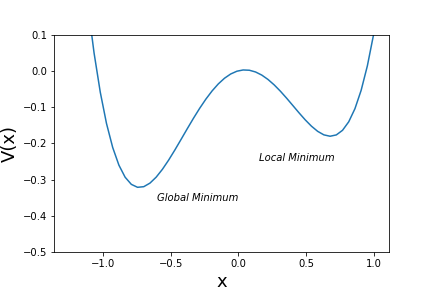
\includegraphics[width=\linewidth]{PotentialWell}
\caption{Potentail well in equation \ref{eq:well} visualized near minima of interest.}
\label{fig:PotentialWell}
\end{figure}

An annealing algorithm was written in fortran to determine the minima. Four different annealing temperature schedules were used to demonstrate the entirety of the annealing process. Three of the schedules were kept at constant temperatures $T=1$, $T=0.4$ and $T=0.1$ while the final schedule linearly decreased from $T=1$ to $T=0.001$ Figures \ref{fig:annealT1}, \ref{fig:annealT04}, \ref{fig:annealT01}, and \ref{fig:anneal_full} show each of the respective schedules.

All of the schedules correctly identified both minima, as well as correctly identifying which minima was the global one. The degree to which they correctly identified the global minimum depended on the schedule used, however. The $T=0.1$ schedule had the highest percentage of walks ending up at the correct value, followed by the full schedule, the $T=0.4$ schedule and the $T=1$ schedules. This was as expected, as lower $T$ would keep a walker close to a minimum for a long time. The full schedule was second best because it was allowed to spend time at other regions during its higher temperature iterations. The success of the pure $T=0.1$ schedule may be attributed to the nature of the step size assigned. By having steps up to a distance of $1$ away, it was always possible for low temp walkers to make the jump between two minima. Had the step size been lower, the low temperature schedule could have had the walker stuck at the local minima, and given the wrong result.

\begin{figure}
\centering
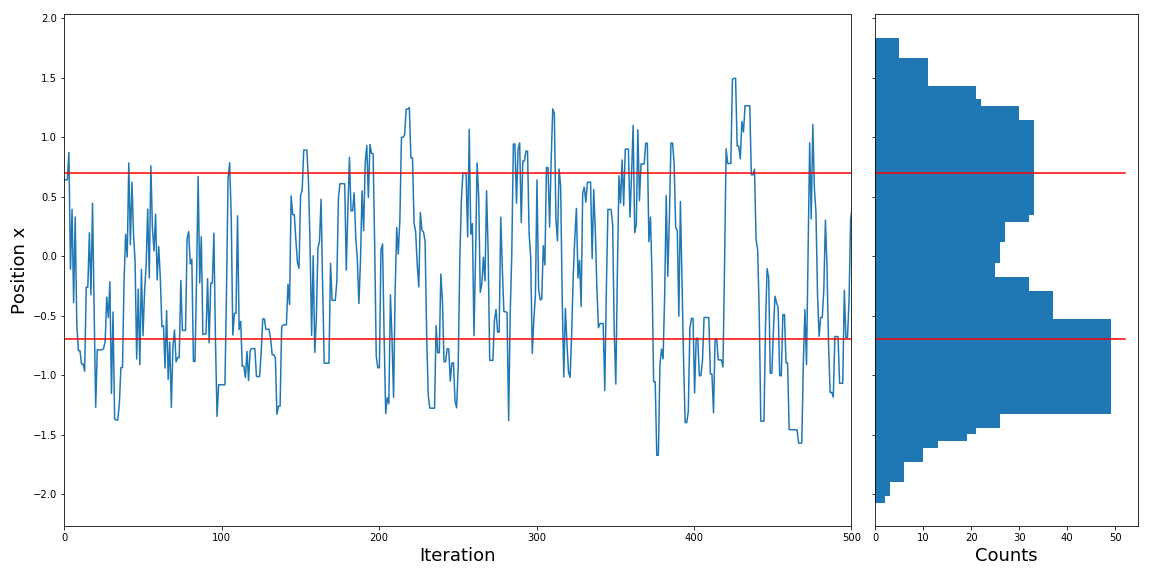
\includegraphics[width=\linewidth]{annealT1}
\caption{Annealing performed on equation \ref{eq:well} to determine local minima. Algorithm was performed at a single temperature $T=1$ for multiple steps. The plot on the left shows each step of the random walker. The plot on the right shows the histogram of walker position.}
\label{fig:annealT1}
\end{figure}

\begin{figure}
	\centering
	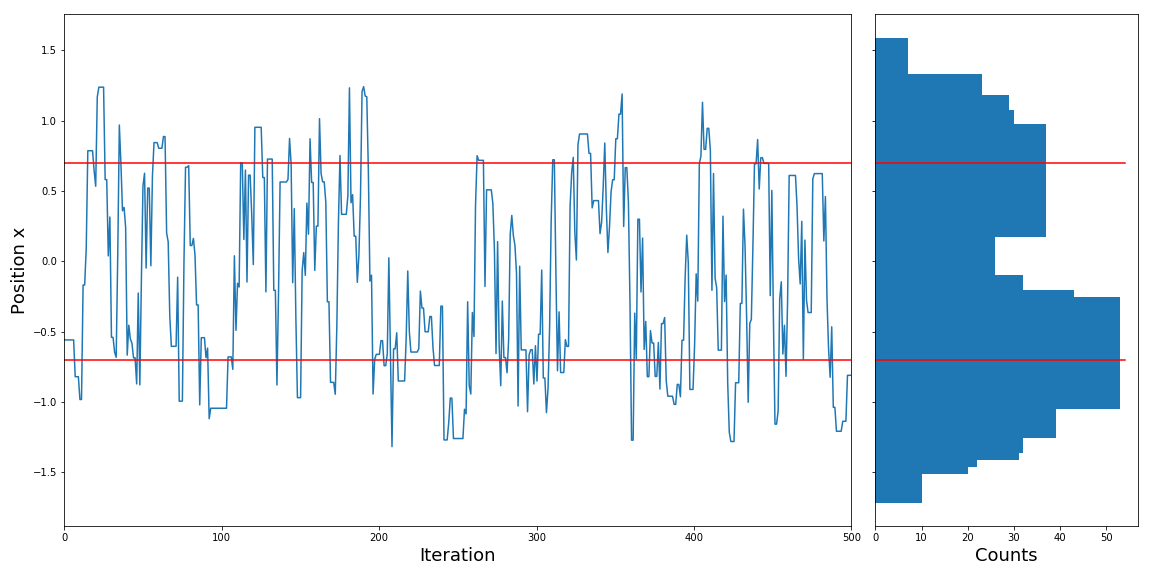
\includegraphics[width=\linewidth]{annealT04}
	\caption{Annealing algorithm at a single temperature $T=0.4$ for multiple steps. The plots are layed out as in \ref{fig:annealT1}.}
	\label{fig:annealT04}
\end{figure}

\begin{figure}
\centering
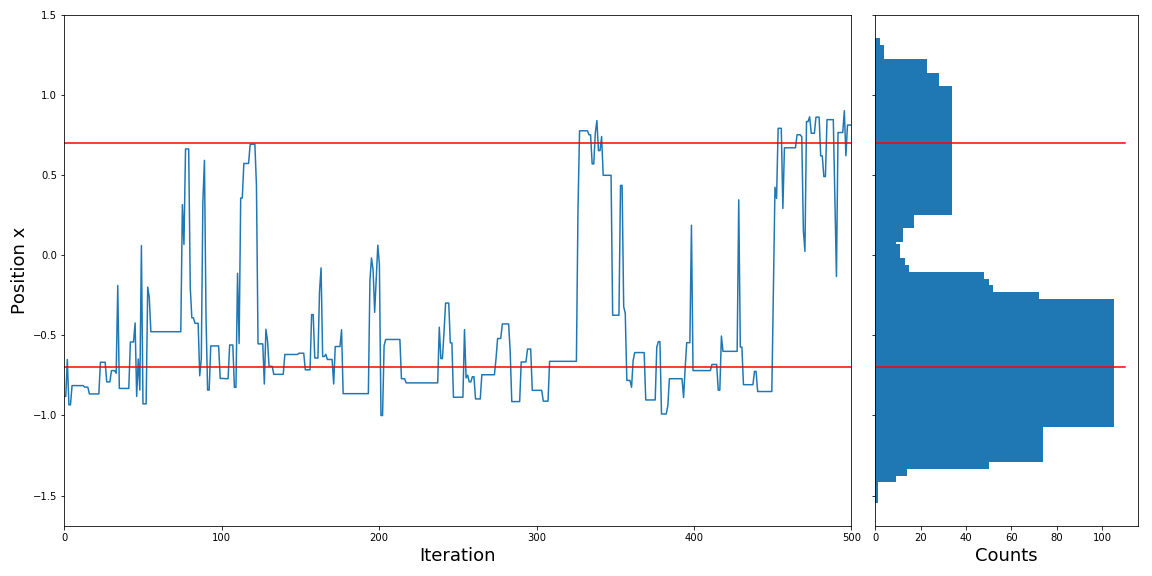
\includegraphics[width=\linewidth]{annealT01}
\caption{Annealing algorithm performed at a single temperature $T=0.001$ for multiple steps. The plots are layed out as in \ref{fig:annealT1}.}
\label{fig:annealT01}
\end{figure}

\begin{figure}
	\centering
	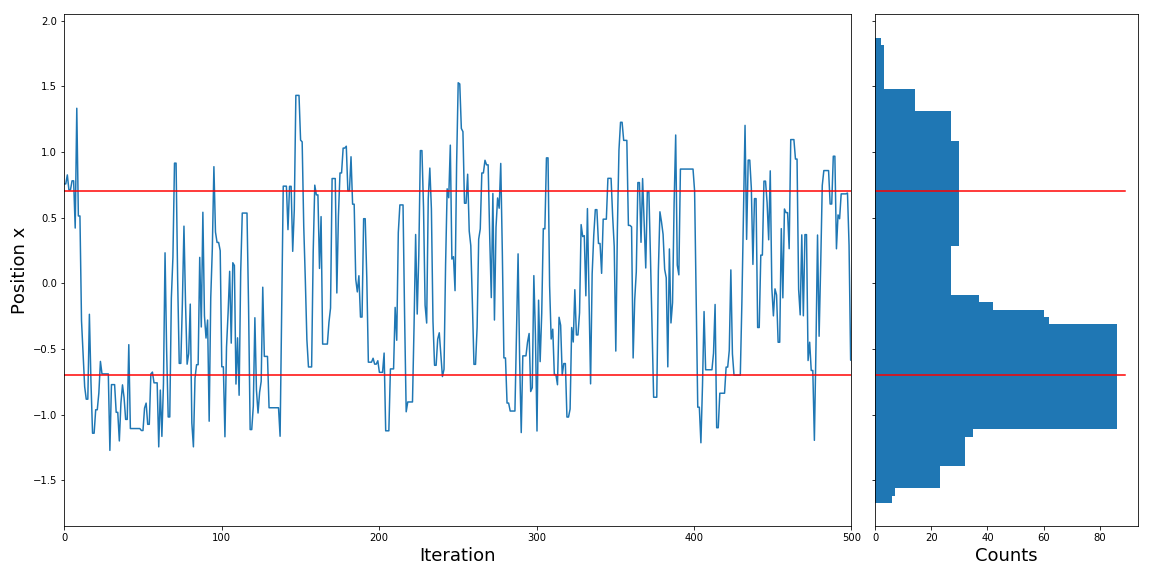
\includegraphics[width=\linewidth]{anneal_full}
	\caption{Location of a global minimum using annealing. A linear temperature schedule from $T=1$ to $T=0.01$ was used. The plots are layed out as in \ref{fig:annealT1}.}
	\label{fig:anneal_full}
\end{figure}

\subsection{Traveling Salesman}
The traveling salesman is a class of mathematical problem dealing with the optimization of path distances. In this example, a salesman must complete a trip to 5 separate cities in as little distance as possible. The distances between cities are shown in table \ref{tab:5cities}. Three different solutions were examined to this problem, nicknamed 'greedy', 'brute-force' and 'annealing'. The greedy method picked a starting city, and then proceeded to its nearest neighbor, repeating this process. The brute-force method calculated every possible path and compared them. The annealing method statistically sampled the path-space by making slight changes to the route and allowing less-optimal paths to be selected with some probability. Figures \ref{fig:greedy_4frames}, \ref{fig:brute_4frames}, and \ref{fig:anneal_4frames} showed each method respectively. 
\begin{table}
\begin{center}
	\begin{tabular}{|c|c|c|c|c|c|}
		\hline
		City $\#$ & 0 & 1 & 2 & 3 & 4 \\
		\hline
		0 & 0. & 3. & 4. & 2. & 7. \\
		\hline
		1 & 3. & 0. & 4. & 6. & 3. \\
		\hline
		2 & 4. & 4. & 0. & 5. & 8. \\
		\hline
		3 & 2. & 6. & 5. & 0. & 6. \\
		\hline
		4 & 7. & 2. & 8. & 6. & 0. \\
		\hline
	\end{tabular}
	\caption{Distances between 5 cities used in a traveling salesman problem.}
	\label{tab:5cities}
\end{center}
\end{table}

Each method was timed using python's timeit library. The timeit function tested the time to run each loop $10^4$ times. The greedy method was run to completion, beginning at city 3. The best route was found to be $3 \to 0 \to 1 \to 4 \to 2$. This code took of $0.0125s$ to run. The brute force method took $0.218s$ to run and from the complete solution found the best route to be $2 \to 3 \to 0 \to 1 \to 4$. The annealing algorithm produced the solution $4 \to 1 \to 0 \to 3 \to 2$ in a time of $0.596s$. The greedy algorithm produced a route of length 16 while the other two produced a length of 13.

Of the three methods given, greedy was the only one to require the selection of a starting city. This matched the real world well, as many businesses have a starting location that a route should start and end at. The greedy method however produced a longer route than the other two methods, making it less reliable. The greedy method excelled in computation time, but the result was undesirable. The other two methods both found the same length 13 route. The brute force method in this case was faster, because even though the annealing method found the correct answer fastest in step 5, it had no way to know this, and continued on for many more instances. As the number of possible cities increases however, annealing would become a better method than brute force. Brute force has a factorial nature, meaning a single city increase has an increasingly negative impact on computation time.

\begin{figure}
\centering
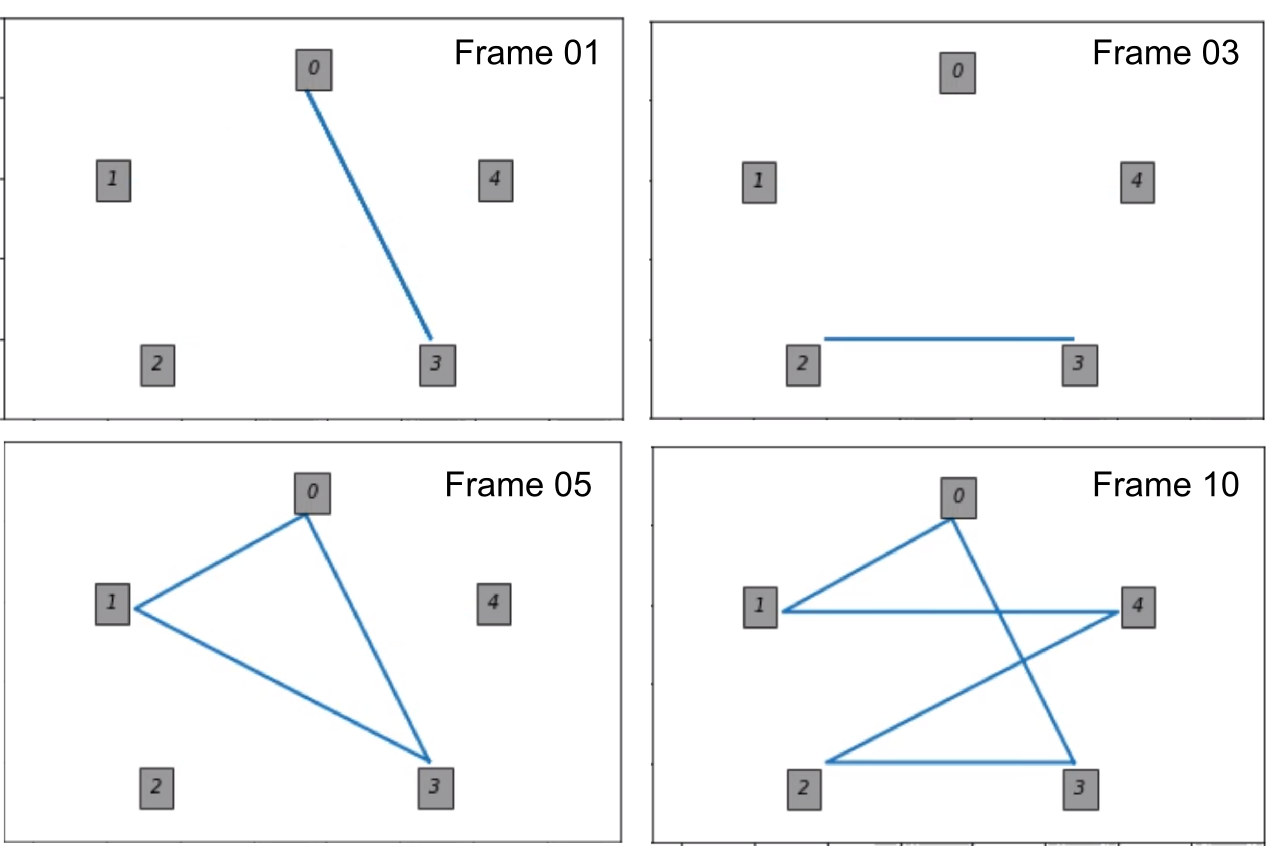
\includegraphics[width=\linewidth]{greedy_4frames}
\caption{Visualization of the greedy method. The method is initialized to start in city 3 in this simulation. In frame 1, the algorithm begins checking the distance from 3 to each other city, starting with 0. Frame 2 shows two steps later, when the algorithm checks the distance of $3 \to 2$ and compares this to the best previous result ($3 \to 0$). In frame 5, the route $3 \to 0$  was selected as the best first segment, and it begins sequentially checking next segments beginning with $0 \to 1$. Frame 10 shows the final result by this method.}
\label{fig:greedy_4frames}
\end{figure}

\begin{figure}
\centering
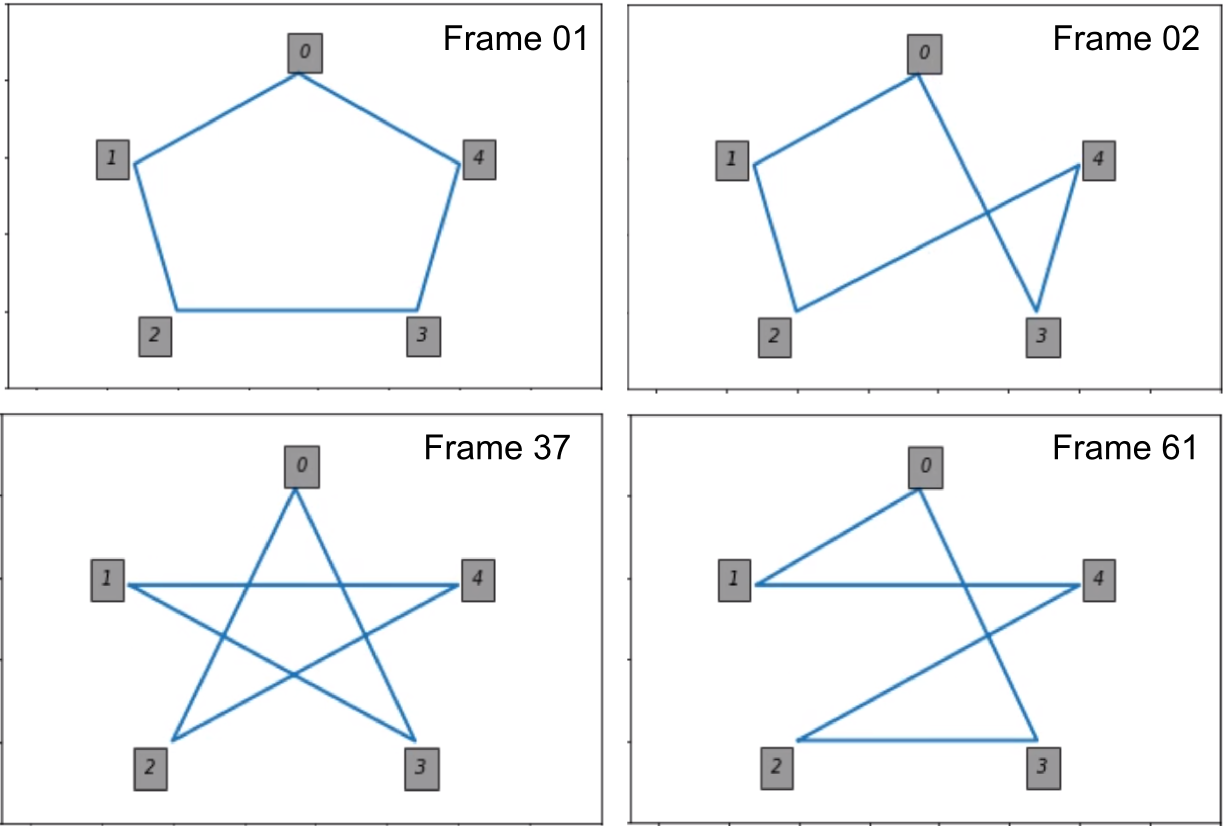
\includegraphics[width=\linewidth]{brute_4frames}
\caption{The brute force method checked every possible permulation of the five city route. Four of the possible permutations were shown here. Frame 61 was found to be the optimal route by this method.}
\label{fig:brute_4frames}
\end{figure}

\begin{figure}
\centering
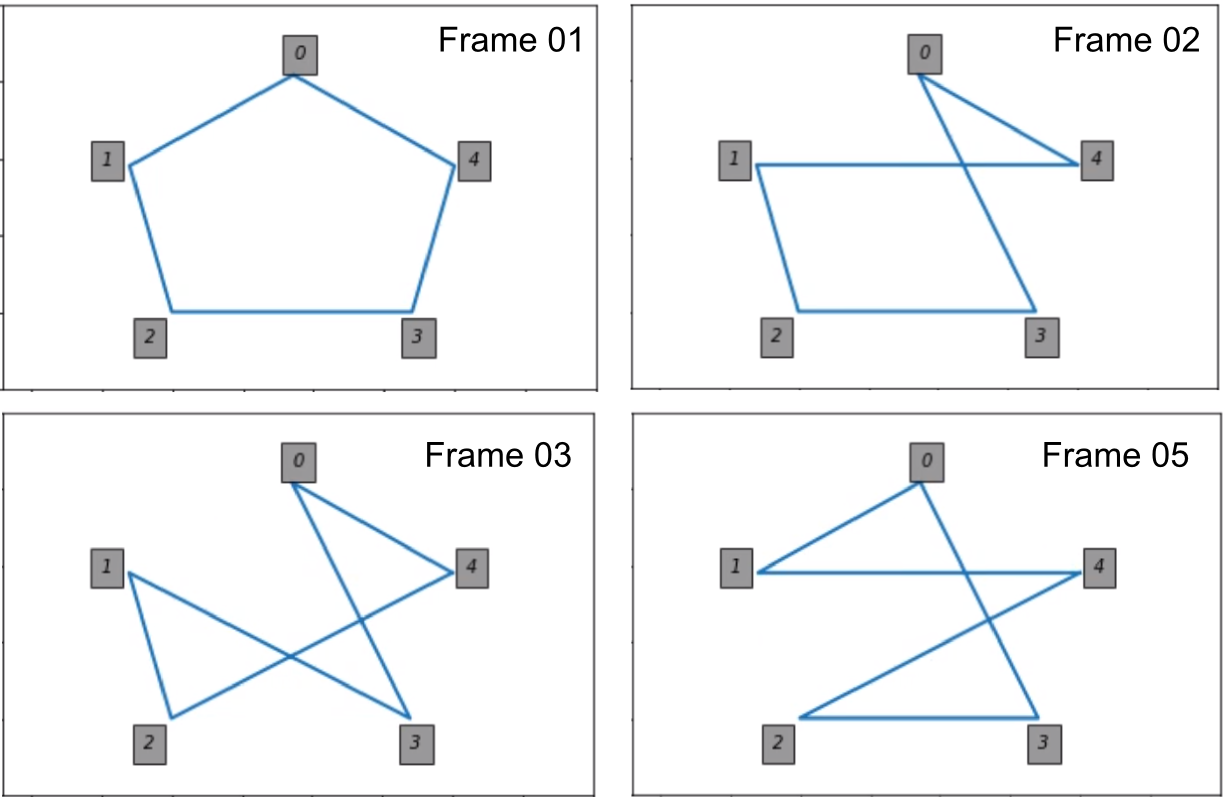
\includegraphics[width=\linewidth]{anneal_4frames}
\caption{Visualization of the annealing method. In frame 01, a simple route was initialized. At each step, a new neighbor configuration was proposed. In frame 02, the positions of cities 0 and 4 were swapped. This configuration was accepted due to being lower total distance. Next, cities 1 and 2 were swapped. At low temperature, this move was accepted, even though it was a longer distance. In frame 05, the cities have found the lowest distance state of the run.}
\label{fig:anneal_4frames}
\end{figure}

\section{Discussion}
Random numbers are often counterintuitive when large statistical phenomena are at play. In the birthday problem it was shown that the probability of two people in a room of thirty having the same birthday are surprisingly high. The initial intuition, that the probability of two people having the same birthday as $1/365$ would lead to a low likelihood for the whole room, was wrong due to the number of combinations of possible people in the room. The problem was checked by generating rooms of people and determining if two individuals shared a birthday. It was found that nearly $70\%$ of rooms had a birthday match present

Gaussians are extremenly common distributions across science, and in physics in particular. The accept/reject method was used to find a gaussian distribution. The result matched the analytical prediction extremely well. This was partially due to the high number of samples taken. The accept/reject method compared the function to a uniform distribution, resulting in many points being rejected. A better distribution, such as a parabola, might reduce the number of draws needed to produce a suitable Gaussian. Once samples were drawn, another distribution was created using sums of numbers drawn from the above Gaussian distribution. The result was taller and narrower, but again appeared to be Gaussian shaped. This is sensible, as the central limit theorem predicts that sums of independently random variables will in turn have a Gaussian distribution.

%MARKOV CHAIN HERE HERE HERE

Besides the accept/reject method, random walkers can be used to create sample distributions. These walkers did not immediately have a desired distribution, as each step was dependent on the last position of the walkers. Over 250 iterations, the distribution had a mean that matched the analytical mean. This is referred to as burn-in. The burn-in can be dependent on the distribution of possible steps for a walker. For this assignment, using $\delta = \pm \sigma$ where $\sigma$ was the standard deviation of the Gaussian,  produced a reasonably quick burn-in. Compared to the accept / reject method, the Markov chain method was significantly faster. This was due to the accept / reject method having a larger number of "wasted" steps with rejection. The accept / reject method has the benefit however of not requiring burn-in, as any number of sample points will obey the target distribution.

The Metropolis-Hastings algorithm required minimal adjustments to the base Metropolis code. The effect of an appropriate proposal distribution was examined for this algorithm. Where earlier in this assignment a uniform distribution was considered acceptable for a proposal distribution, this example showed that a proposal distribution more closely matching the shape of the target distribution produced a better mixed Markov chain. In effect, this meant that the $\chi^2$ proposal distribution required a lower burn-in time than the uniform distribution to achieve a good sampling. 
 
\section{Conclusion}



\begin{thebibliography}{00}
	\bibitem{ouyed}
	Ouyed and Dobler, PHYS 581 course notes, Department of Physics and Astrophysics, University of Calgary (2016).
	\bibitem{NR}
	W. Press et al., \emph{Numerical Recipes} (Cambridge University Press, 2010) 2nd. Ed.
	\bibitem{Code}
	C. Hass and J. Burniston, MCMC Hill Climbing. Jupyter notebook, 2018.
\end{thebibliography}

\section{Appendix}
For access to the source codes used in this project, please visit \url{https://github.com/Tsintsuntsini/PHYS_581} for a list of files and times of most recent update.
	
\end{document}